\documentclass[fleqn, a4paper, 11pt, oneside]{amsart}
%\usepackage[top = 2cm, bottom = 1cm, left = 1cm, right = 1cm]{geometry}
\usepackage{exsheets, tasks}
\usepackage{amsmath, amssymb, amsthm} %standard AMS packages
\usepackage{marginnote} %marginnotes
\usepackage{gensymb} %miscellaneous symbols
\usepackage{commath} %differential symbols
\usepackage{xcolor} %colours
\usepackage{cancel} %cancelling terms
\usepackage[free-standing-units, space-before-unit]{siunitx} %formatting units
\usepackage{tikz, pgfplots} %diagrams
\usetikzlibrary{calc, hobby, patterns, intersections, decorations.markings}
\usepackage{graphicx} %inserting graphics
\usepackage{hyperref} %hyperlinks
\usepackage{datetime} %date and time
\usepackage{ulem} %underline for \emph{}
\usepackage{xfrac} %inline fractions
\usepackage{enumerate,enumitem} %numbered lists
\usepackage{float} %inserting floats
\usepackage{circuitikz}[american voltages, american currents] %circuit diagrams

\newcommand\numberthis{\addtocounter{equation}{1}\tag{\theequation}} %adds numbers to specific equations in non-numbered list of equations

\newcommand{\AxisRotator}[1][rotate=0]{
	\tikz [x=0.25cm,y=0.60cm,line width=.2ex,-stealth,#1] \draw (0,0) arc (-150:150:1 and 1);%
} %rotation symbols on axes

\theoremstyle{definition}
\newtheorem{example}{Example}
\newtheorem{definition}{Definition}

\theoremstyle{theorem}
\newtheorem{theorem}{Theorem}

\newcommand{\curl}{\mathrm{curl\,}}

\makeatletter
\@addtoreset{section}{part} %resets section numbers in new part
\makeatother

\renewcommand{\thesubsection}{(\arabic{subsection})}
\renewcommand{\thesection}{(\arabic{section})}

%section headings on left
\makeatletter
\def\specialsection{\@startsection{section}{1}%
	\z@{\linespacing\@plus\linespacing}{.5\linespacing}%
	%  {\normalfont\centering}}% DELETED
	{\normalfont}}% NEW
\def\section{\@startsection{section}{1}%
	\z@{.7\linespacing\@plus\linespacing}{.5\linespacing}%
	%  {\normalfont\scshape\centering}}% DELETED
	{\normalfont\scshape}}% NEW
\makeatother

%forces newline after subsection
\makeatletter
\def\subsection{\@startsection{subsection}{3}%
	\z@{.5\linespacing\@plus.7\linespacing}{.1\linespacing}%
	{\normalfont\itshape}}
\makeatother

\settasks{counter-format = tsk[1].}

\SetupExSheets{solution/print = true}

%opening
\title{Physics 2 : Assignment 11}
\author
{
	Aakash Jog\\
	ID : 989323563
}
\date{\formatdate{3}{6}{2015}}

\begin{document}

\tikzset{->-/.style={decoration={
  markings,
  mark=at position #1 with {\arrow{>}}},postaction={decorate}}}

\maketitle
%\setlength{\mathindent}{0pt}

\begin{question}
	A square loop of side $a$ is mounted on a vertical shaft and rotated at angular velocity $\omega$.
	A uniform magnetic field $\overrightarrow{B}$ is pointing to the right.
	Find the $\varepsilon(t)$ for this alternating current generator.
\end{question}

\begin{solution}
	Let the angle between the $\overrightarrow{A}$, the area vector of the loop, and $\overrightarrow{B}$ be $\theta$.\\
	Therefore, by Faraday's Law,
	\begin{align*}
		\varepsilon(t) &= -\dod{\Phi_B}{t}\\
		&= -\dod{}{t}\left( \overrightarrow{A} \cdot \overrightarrow{B} \right)\\
		&= -\dod{}{t}\left( A B \cos \theta \right)\\
		&= -A B \dod{(\cos \theta)}{t}\\
		&= -A B \dod{(\cos \omega t + \varphi)}{t}\\
		&= A B \omega \sin \omega t + \varphi\\
		&= a^2 B \omega \sin \omega t + \varphi
	\end{align*}
\end{solution}

\begin{question}
	A metal disk of radius $a$ is rotating at angular velocity $\omega$ about a vertical axis, through a uniform field $\overrightarrow{B}$ pointing upwards.
	A circuit is made by connecting one end of a resistor $R$ to the axle and the other end to a sliding contact, which touches the outer edge of the disk.
	Find the current in the resistor.
\end{question}

\begin{solution}
	Consider an elemental rod of length $\dif l$ at a distance $l$ from the centre of the disk.\\
	As it is moving,
	\begin{align*}
		\dif \varepsilon &= B v \dif l\\
		&= B \omega l \dif l\\
		\therefore \varepsilon &= \int\limits_{0}^{a} B \omega l \dif l\\
		&= B \omega \frac{a^2}{2}
	\end{align*}
	Therefore,
	\begin{align*}
		\varepsilon &= I R\\
		\therefore \frac{B \omega a^2}{2} &= I R\\
		\therefore I &= \frac{B \omega a^2}{2 R}
	\end{align*}
\end{solution}

\begin{question}
	A square loop of wire, of side $a$ lies on a table, at distance $s$ from a very long straight wire, which carries a current $I$, as shown.
	\begin{figure}[H]
		\begin{tikzpicture}
			\def\a{2};
			\def\s{1};
			\def\l{6};

			\draw[->- = 0.5] (-\l/2,0) -- (\l/2,0) node [midway, below] {$I$};

			\draw (-\a/2,\s) rectangle (\a/2,\s + \a);

			\begin{scope}
				\draw[xshift = -20, decorate, decoration = {brace}] (-\a/2,\s) -- ++(90:\a) node [midway, left] {$a$};
				\draw[xshift = -20, decorate, decoration = {brace}] (-\a/2,0) -- ++(90:\s) node [midway, left] {$s$};
			\end{scope}
		\end{tikzpicture}
	\end{figure}
	\begin{enumerate}
		\item Find the flux of the magnetic field through the loop.
		\item
			If someone now pulls the loop directly away from the wire at speed $v$, what emf is generated?
			In what direction does the current flow?
		\item What if the loop is pulled to the right at speed $v$ instead of away?
	\end{enumerate}
\end{question}

\begin{solution}
	\begin{enumerate}
		\item
			Let $\overrightarrow{A}$ be the area vector of the loop.
			Let it be directed outwards.\\
			By the right hand thumb rule, $\overrightarrow{B}$ due to the wire is also directed outwards.\\
			Consider an elemental strip of length $a$ and breadth $\dif h$, at a distance $h$ from the wire.\\
			Let its area vector be $\dif A$, directed outwards.\\
			Therefore, the magnetic flux through it is,
			\begin{align*}
				\dif \Phi_B &= \dif \overrightarrow{A} \cdot \overrightarrow{B}\\
				&= a \dif h \cdot \frac{\mu_0 I}{2 \pi h}\\
				\therefore \Phi_B &= \frac{\mu_0 I a}{2 \pi} \int\limits_{s}^{s + a} \frac{\dif h}{h}\\
				&= \frac{\mu_0 I a}{2 \pi} \ln\left( \frac{s + a}{s} \right)\\
				&= \frac{\mu_0 I a}{2 \pi} \ln\left( 1 + \frac{a}{s} \right)
			\end{align*}
		\item
			By Faraday's Law,
			\begin{align*}
				\varepsilon &= -\dod{\Phi_B}{t}\\
				&= -\dod{}{t}\left( \frac{\mu_0 I a}{2 \pi} \ln \left( 1 + \frac{a}{s} \right) \right)\\
				&= -\frac{\mu_0 I a}{2 \pi} \dod{}{t}\left( \ln \left( \frac{s + a}{s} \right) \right)\\
				&= -\frac{\mu_0 I a}{2 \pi} \dod{}{t}\left( \ln(s + a) - \ln s \right)\\
				&= -\frac{\mu_0 I a}{2 \pi} \left( \frac{1}{s + a} \dod{s}{t} - \frac{1}{s} \dod{s}{t} \right)\\
				&= \frac{\mu_0 I a}{2 \pi} \left( \frac{v}{s} - \frac{v}{s + a} \right)
			\end{align*}
			By Lenz's Law, the induced current is such that the induced magnetic field opposes its own cause.\\
			As the loop is pulled away, the magnetic field reduces in the outwards direction, i.e. increases in the inwards direction.\\
			Therefore, the induced current is in a direction such that the induced magnetic flux is directed outwards.\\
			Therefore, the induced current is anti-clockwise.
		\item
			If the loop is pulled to the right instead of away, as the wire is infinite, the magnetic flux through the loop is constant.\\
			Therefore, by Faraday's Law,
			\begin{align*}
				\varepsilon &= -\dod{\Phi_B}{t}\\
				&= 0
			\end{align*}
	\end{enumerate}
\end{solution}

\begin{question}
	A square loop is cut out of a thick sheet of aluminium.
	It is then placed so that the top portion is in a uniform magnetic field $\overrightarrow{B}$, pointing inwards, and allowed to fall under gravity, as shown.
	\begin{figure}[H]
		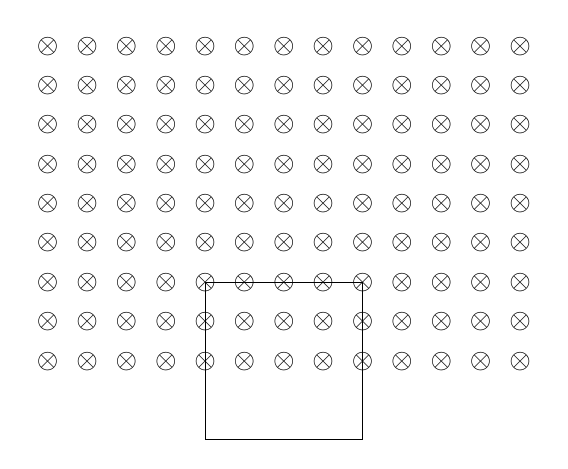
\begin{tikzpicture}
			\def\a{2};
			\def\l{6};
			\def\h{4};

			\foreach \x in {0,0.5,...,\l}
			{
				\foreach \y in {0,0.5,...,\h}
				{
					\node at (\x,\y) {$\otimes$};
				}
			}

			\draw (\l/2 - \a/2,-\a/2) rectangle (\l/2 + \a/2,\a/2);
		\end{tikzpicture}
	\end{figure}
	If the magnetic field is $1 \tesla$, find the terminal velocity of the loop in $\si{\metre\per\second}$.
	Find the velocity of the loop as a function of time.
	How long does it take, in seconds, to reach, say $90\%$ of the terminal velocity?
	What would happen is you cut a tiny slit in the ring?\\
	Note: The dimensions of the loop cancel out.
	Determine the actual numbers using the following values.
	\begin{itemize}
		\item Resistivity of aluminium: $\rho = 2.8 \times 10^{-8} \si{\ohm\metre}$
		\item Mass density of aluminium: $\eta = 2.7 \times 10^3 \si{\kg\per\metre\cubed}$
	\end{itemize}
\end{question}

\begin{solution}
	Let the length of the side of the loop be $l$.\\
	Let the cross-sectional area of the loop be $A$.\\
	Let the velocity of the loop be $v$.\\
	Therefore,
	\begin{align*}
		\varepsilon &= B l v\\
		\therefore I R &= B l v\\
		\therefore I &= \frac{B l v}{R}
	\end{align*}
	Therefore,
	\begin{align*}
		F_B &= I l B\\
		&= \frac{B l v}{R} l B\\
		&= \frac{B^2 l^2 v}{R}\\
		&= \frac{B^2 l^2 v}{4 \frac{\rho l}{A}}\\
		&= \frac{A B^2 l^2 v}{4 \rho l}
	\end{align*}
	When the loop reaches terminal velocity,
	\begin{align*}
		F_g &= F_B\\
		\therefore m g &= \frac{A B^2 l^2 v_t}{4 l \rho}\\
		\therefore v_t &= \frac{4 l \rho m g}{A B^2 l^2}\\
		&= \frac{4 l \rho (4 A l \eta) g }{A B^2 l^2}\\
		&= \frac{16 l^2 A \rho \eta g}{A B^2 l^2}\\
		&= \frac{16 \rho \eta g}{B^2}
	\end{align*}
	Therefore, as $B = 1 \tesla$, $\rho = 2.8 \times 10^{-8} \si{\ohm\metre}$, $\eta = 2.7 \times 10^3 \si{\kg\per\metre\cubed}$,\\
	\begin{align*}
		v &= \frac{(16) \left( 2.8 \times 10^{-8} \right) \left( 2.7 \times 10^3 \right) g}{1^2}\\
		&= (16) (2.8) (2.7) (g) \left( 10^{-5} \right)\\
		&= 120.96 g \times 10^{-5} \si{\metre\per\second}
	\end{align*}
	\begin{align*}
		\dod{v}{t} &= a\\
		&= g - \frac{A B^2 l^2 v}{4 m \rho l}\\
		&= g - \frac{A B^2 l^2 v}{4 (4 A l \eta) \rho l}\\
		&= g - \frac{A B^2 l^2 v}{ 16 A l^2 \rho \eta}\\
		&= g - \frac{B^2 v}{16 \rho \eta}\\
		\therefore \frac{\dif v}{g - \frac{B^2 v}{16 \rho \eta}} &= \dif t\\
		\therefore \int\limits_{0}^{v} \frac{\dif v}{g - \frac{B^2 v}{16 \rho \eta}} &= \int\limits_{0}^{t} \dif t
	\end{align*}
	Therefore, integrating,
	\begin{align*}
		\therefore -\frac{16 \rho \eta}{B^2} \left( \ln\left( g - \frac{B^2 v}{16 \rho \eta} \right) - \ln g \right) &= t\\
		\therefore \ln\left( \frac{g - \frac{B^2 v}{16 \rho \eta}}{g} \right) &= -\frac{B^2 t}{16 \rho \eta}\\
		\therefore \frac{g - \frac{B^2 v}{16 \rho \eta}}{g} &= e^{-\frac{B^2 t}{16 \rho \eta}}\\
		\therefore \frac{B^2 v}{16 \rho \eta} &= g - g e^{-\frac{B^2 t}{16 \rho \eta}}\\
		\therefore v &= \frac{16 \rho \eta g}{B^2} \left( 1 - e^{-\frac{B^2 t}{16 \rho \eta}} \right)\\
		&= v_t \left( 1 - e^{-\frac{B^2 t}{16 \rho \eta}} \right)
	\end{align*}
	Therefore, if $v = 0.9 v_t$,
	\begin{align*}
		0.9 v_t &= v_t \left( 1 - e^{-\frac{B^2 t}{16 \rho \eta}} \right)\\
		\therefore 0.9 &= 1 - e^{-\frac{B^2 t}{16 \rho \eta}}\\
		\therefore e^{-\frac{B^2 t}{16 \rho \eta}} &= 0.1\\
		\therefore -\frac{B^2 t}{16 \rho \eta} &= \ln 0.1\\
		\therefore t &= -\frac{16 \rho \eta \ln(0.1)}{B^2}
	\end{align*}
	If a tiny slit is cut in the ring, there will be no current flowing in the ring.\\
	Therefore, there will will be no resisting force.\\
	Hence, the ring will fall under gravity only.
\end{solution}

\end{document}
